\section{Scientific question}
\label{sec:question}
How does atomic-scale carbon architecture control stiffness, strength, failure strain, energy absorption, flaw sensitivity, crack initiation and propagation, damage localisation, and the transition between abrupt and progressive fracture? We treat structural complexity---hierarchy in particular---as a controlled experimental variable rather than as a presumed advantage. Null results, trade-offs, unstable candidates and counter-examples are reported as results in their own right. All statements below refer to the behaviour of one classical model (screened second-generation REBO, \rebo{}) under athermal quasi-static (AQS) loading; none of the simulated structures is claimed to be synthesizable, and no simulation is described as an experiment.

\section{Reference-image interpretation and inferred design language}
\label{sec:images}
The five reference images (Fig.~\ref{fig:images}) were examined without assuming a common object. They are not treated as templates; instead, transferable geometric and topological principles were extracted and each was mapped to an atomistic realisation in graphene-derived carbon. The interpretation is stored as an editable document (\texttt{analysis/image\_interpretation.json}) that the application exposes for modification and regeneration.

\begin{figure}[H]\centering
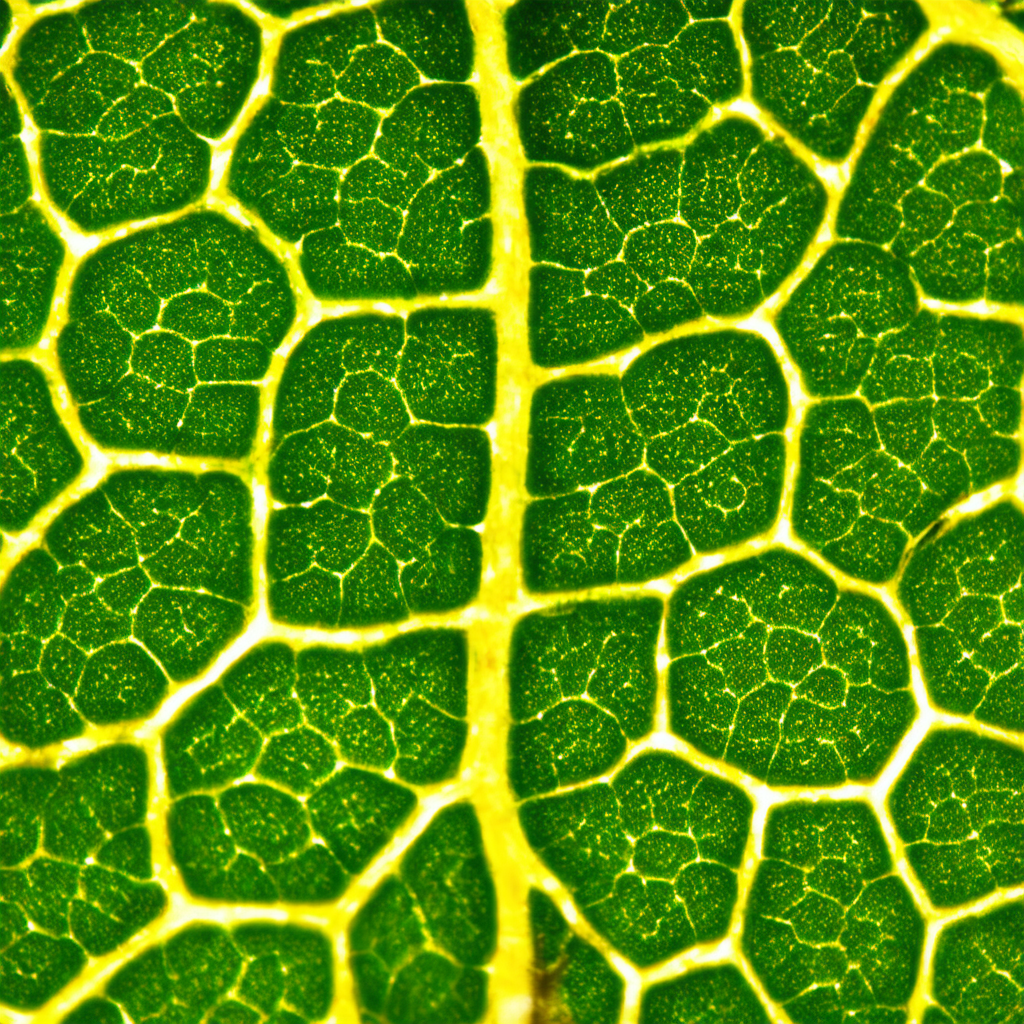
\includegraphics[width=0.19\textwidth]{../reference_images/image_grid_20240721_220650.png}\hfill
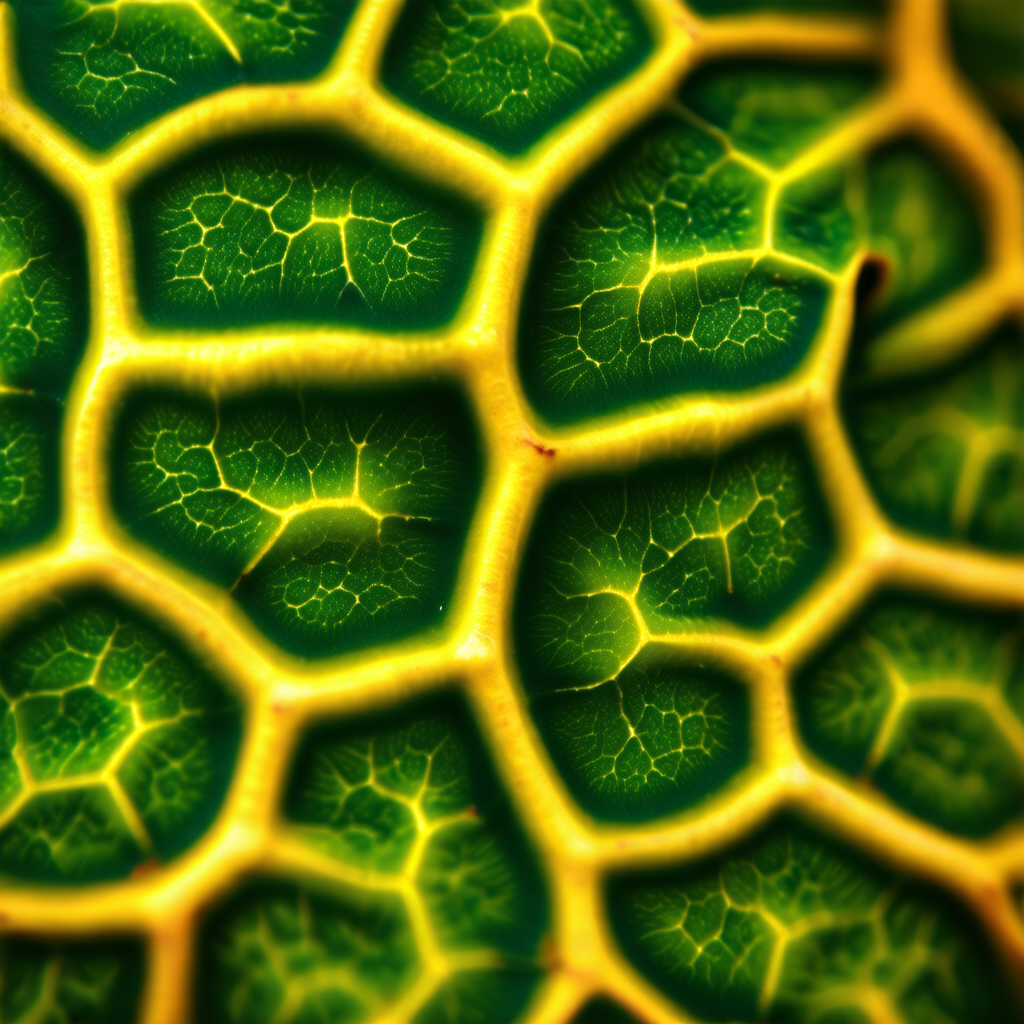
\includegraphics[width=0.19\textwidth]{../reference_images/image_grid_2-of-16__20240721_210804.png}\hfill
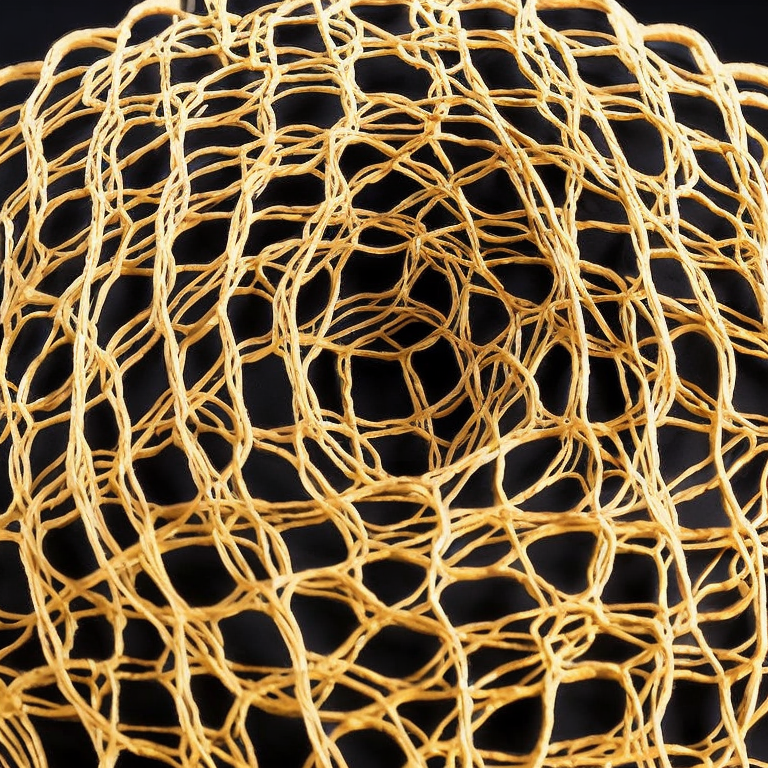
\includegraphics[width=0.19\textwidth]{../reference_images/image_grid_2-of-3__20240721_061946.png}\hfill
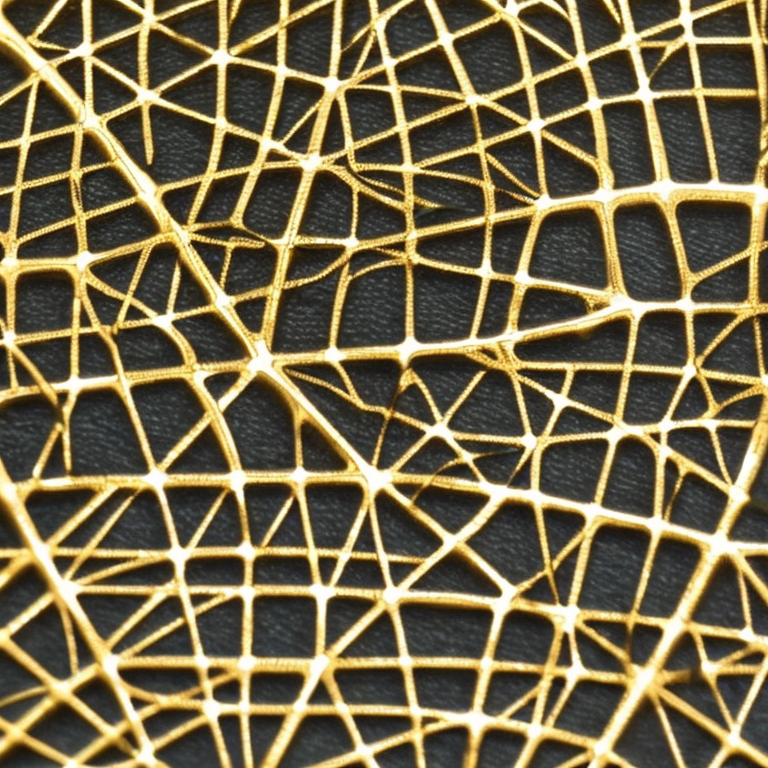
\includegraphics[width=0.19\textwidth]{../reference_images/image_grid_7-of-9__20240721_063700.png}\hfill
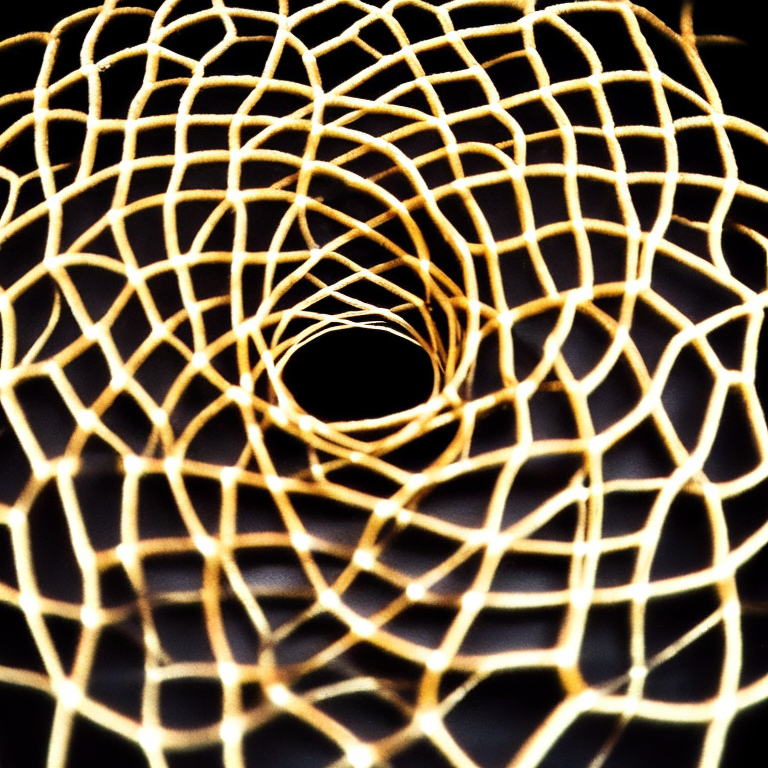
\includegraphics[width=0.19\textwidth]{../reference_images/image_grid_0-of-3__20240721_061945.png}
\caption{Reference images (left to right): hierarchical leaf venation (img1); closed-cell walls enclosing a fine open network (img2); disordered layered fibre net (img3); rectilinear crossing struts (img4); nested rings around a central void with a size gradient (img5).}
\label{fig:images}
\end{figure}

\begin{table}[H]\centering\footnotesize
\caption{Design principles extracted from the reference images, their atomistic realisation, main assumption and a plausible alternative reading.}
\label{tab:principles}
\setlength{\tabcolsep}{4pt}
\begin{tabular}{p{0.45cm}>{\raggedright\arraybackslash}p{2.1cm}>{\raggedright\arraybackslash}p{2.2cm}>{\raggedright\arraybackslash}p{4.6cm}>{\raggedright\arraybackslash}p{2.4cm}>{\raggedright\arraybackslash}p{2.4cm}}
\toprule
 & Principle & Motivating feature & Atomistic realisation & Assumption & Alternative\\
\midrule
P1 & nested hierarchy & vein widths at 3--4 scales (img1); coarse walls + fine net (img2); rings within rings (img5) & nanomesh with fine pores (period $p_1$) inside domains bounded by wider ``vein'' ligaments (width $W_2$, domain $D_2$); optional third level ($W_3$, $D_3$) & ligaments $\gtrsim 5$\,\AA{} remain stable sp$^2$ carbon; coarse scale limited by the supercell & graded ligament widths without domains; hierarchical defects\\
P2 & redundancy / loops & closed loops at every level (img1); overlaid nets (img3) & cyclomatic number of the ligament graph; closed-cell vs open patterns at equal porosity & loops counted on the relaxed bond graph & layering not accessible in one sheet\\
P3 & compart\-mentalisation & thick walls isolate cells (img2) & vein network of the two-level mesh; do cracks stop at veins? & vein width sets barrier strength & walls may act as stress concentrators\\
P4 & anisotropy & midrib direction (img1); crossing struts (img4) & slits / elliptical pores at $0/45/90^\circ$; strut families; zigzag vs armchair lattice & uniaxial loading along $x$ & lattice chirality as an atomistic anisotropy\\
P5 & scale separation & ratio $\sim$5--10 between levels (img2) & domain size $D_2$ at fixed $p_1$ (ratios 2--5) & cell must hold several domains & continuous (graded) separation\\
P6 & disorder & irregular cells (img3) & jittered / size-dispersed pore lattices; periodic Voronoi networks with tunable regularity; multiple seeds & quenched disorder & disorder of ligament width\\
P7 & tortuous paths & curved fibres (img3) & Voronoi networks, staggered lattices; descriptor tortuosity & measured on bond graph & wavy slits\\
P8 & straight through-going paths & lines spanning the field (img4) & strut lattices with/without a family along the load; slits parallel to the load & periodic continuation & staggered struts\\
P9 & node connectivity & 3--4 lines meeting at nodes (img4) & $0/60/120^\circ$ (6-connected) vs $0/90^\circ$ (4-connected) vs $30/90/150^\circ$ (no strut along load) & stretching-dominated plates & masked by node stress concentration\\
P10 & gradients & shrinking cells (img5) & pore-size gradient along $x$ or radial & gradient wavelength limited by cell & ligament-width gradient\\
P11 & nesting around a flaw & rings around a hole (img5) & hole + concentric rings of small pores vs bare hole vs hole + uniform far-field pores at matched porosity & halo changes the hole stress field & rings add crack nuclei\\
\bottomrule
\end{tabular}
\end{table}

\section{Generated carbon architecture space}
\label{sec:space}
All candidates are explicit carbon atoms in orthorhombic periodic supercells ($x$ and $y$ periodic, vacuum along $z$), represented as ASE \texttt{Atoms} objects~\cite{ase} that carry generator family, parameters and random seed in their metadata. Structures are derived from a rectangular graphene sheet at the \rebo{} equilibrium lattice constant ($a_0 = 2.4602$\,\AA) by atom removal (pores, slits, cracks, vacancies), followed by iterative pruning of atoms with fewer than two neighbours, removal of disconnected fragments, and relaxation. Ten generator families instantiate the principles of Table~\ref{tab:principles}: \texttt{pristine}, \texttt{nanomesh\_single}, \texttt{nanomesh\_hier} (two- and three-level nested meshes), \texttt{voronoi\_network}, \texttt{slit\_array}, \texttt{strut\_lattice}, \texttt{graded\_pores}, \texttt{ring\_around\_hole}, \texttt{precrack} and \texttt{vacancies}. For every controlled comparison the free size parameter of each family is adjusted by bisection so that the porosity of the generated structure matches a target ($\phi = 0.20\pm0.01$ unless stated), which fixes carbon mass and footprint across architectures. Descriptors are measured on the relaxed structures (not taken from generator parameters): porosity, areal density, coordination statistics, fraction of two-coordinated edge atoms, bond-graph cyclomatic number per atom (redundancy), load-path tortuosity (shortest periodic bond path across $x$ divided by $L_x$), pore-size and ligament-width distributions from Euclidean distance transforms of a periodic raster, the minimum load-bearing solid fraction across the loading direction (bottleneck), a structure-tensor anisotropy index, and hierarchy metrics (number of distinct pore/ligament scales, scale ratio, coarse-ligament solid fraction).

\subsection{Hierarchy as a controlled multivariable design axis}
The hierarchy ladder (Fig.~\ref{fig:space}) spans, at matched porosity and footprint (120\,\AA{} cells): single-scale meshes with fine (12\,\AA), reference (16\,\AA) and coarse (32\,\AA) periods, the coarse level alone (square pores on the 40\,\AA{} vein grid), two-level nested meshes with domain sizes 24/40/60\,\AA{} (scale ratios 2, 3.3, 5 relative to the 12\,\AA{} fine period) and vein widths 4/8/12\,\AA, and a three-level mesh (10\,\AA{} period, 30\,\AA{} domains with 5\,\AA{} veins, 120\,\AA{} domains with 12\,\AA{} veins). Hierarchy depth, scale ratio, inter-level ligament width, inter-level connectivity (fine ligaments attach to veins), and the organisation of hierarchy relative to the load are therefore separately variable.

\section{Force field}
\label{sec:ff}
The authoritative production potential is the screened second-generation REBO potential for carbon (\rebo{}, ``Rebo2Scr'')~\cite{brenner2002,pastewka2008,pastewka2013} in the parameterisation and implementation of Atomistica 1.2.7~\cite{atomistica} (default parameters: $C_\mathrm{min}=1$, $C_\mathrm{max}=2$, dihedral term off, default $P_{CC}$, $F_{CC}$ tables). The energy is
\begin{equation}
E=\sum_{i<j} f^{ar}_{ij}\left[V_R(r_{ij})+\bar b_{ij}V_A(r_{ij})\right],\qquad
\bar b_{ij}=\tfrac12\left(b_{ij}+b_{ji}+F_{CC}(N^t_i,N^t_j,N^{conj}_{ij})\right),
\end{equation}
\begin{equation}
b_{ij}=\Big(1+\sum_{k\neq i,j} f^{bo}_{ik}\,g(\cos\theta_{jik},N^t_i)+P_{CC}(N^H_i,N^C_i)\Big)^{-1/2},
\end{equation}
with the screened cut-off functions $f^{x}_{ij}=(1-f^{in}_{ij})S_{ij}f^{x}(r_{ij})+f^{in}_{ij}$ ($x\in\{ar,bo,nc\}$) and the elliptical screening function $S_{ij}=\prod_k S(C_{ijk})$, $S(C)=\exp[-((C_\mathrm{max}-C)/(C-C_\mathrm{min}))^2]$ for $C_\mathrm{min}<C<C_\mathrm{max}$ (0 below, 1 above), $C_{ijk}=[2(x_{ik}+x_{jk})-(x_{ik}-x_{jk})^2-1]/[1-(x_{ik}-x_{jk})^2]$, $x_{ik}=r_{ik}^2/r_{ij}^2$. Cut-off radii are 1.95--2.25\,\AA{} (inner), 2.179--2.820\,\AA{} (pair), 1.866--2.758\,\AA{} (bond order) and 1.217--4.000\,\AA{} (neighbour count / conjugation). No parameter, screening function or cut-off was modified. Every run record stores the potential name, implementation, version, literature references, source commit, a SHA-256 checksum of the published parameters and tables, and the units.

\section{Implementation}
\label{sec:impl}
\textbf{TorchRebo2Scr.} A GPU-native PyTorch~\cite{pytorch} implementation was written by transcribing the Atomistica kernel (\texttt{bop\_kernel\_rebo2.f90} with the \texttt{SCREENING}, \texttt{NUM\_NEIGHBORS} and trigonometric cut-off options, \texttt{rebo2\_func.f90}, \texttt{rebo2\_db.f90}, \texttt{rebo2\_default\_tables.f90}, \texttt{table2d.f90}, \texttt{table3d.f90}). The angular spline coefficients and the bicubic/tricubic table coefficients are obtained by solving the same linear systems as the Fortran code; the single-precision Fortran literals of the angular knot values are reproduced deliberately (without this detail the two implementations differ by $10^{-8}$\,eV/atom). Energies are evaluated with dense, padded neighbour tensors ($[N,M]$ pairs within 4.0\,\AA{}+skin for screening and coordination, $[N,M_b]$ pairs within 2.82\,\AA{}+skin for pair energies and bond order, $[N,M,M]$ screening triplets, $[N,M_b,M_b]$ angular triplets); forces are exact gradients by automatic differentiation, $\mathbf F=-\partial E/\partial\mathbf R$, and the virial is $\partial E/\partial\boldsymbol\varepsilon$ for an affine strain of all pair vectors. Per-atom energies (half of each pair energy) and per-atom virials (pair-vector decomposition) are available for visualisation. Value caps of the neighbour counts ($N\le4$, $N^t\le3$, $N^{conj}\le8$) are implemented with straight-through gradients so that forces coincide with Atomistica's even in over-coordinated environments. Degenerate screening geometries ($k$ projecting exactly onto $i$ or $j$, contribution exactly 1) are excluded from the product to keep the float32 backward pass free of $0/0$. The engine runs on \texttt{mps} (Apple GPU, float32), \texttt{cuda} (float32/64) and \texttt{cpu} (float32/64) with automatic backend detection; the campaign used MPS float32 (``fast discovery mode''); CPU float64 is the ``reference mode''.

\textbf{Neighbour lists.} Pair lists are built with a cell-list algorithm (ASE \texttt{primitive\_neighbor\_list}, $O(N)$), padded to dense tensors, sorted by distance so that the short list is a prefix of the long list, and equipped with reverse-pair indices for periodic images. A Verlet skin of 0.3\,\AA{} with a half-skin displacement criterion (checked every FIRE iteration relative to the affine image of the build-time positions) triggers rebuilds. The optimised list is validated against brute-force enumeration (TEST~9).

\textbf{Batching.} Several independent structures are concatenated into one ``super-system'' (per-atom structure index, per-structure cells and strain tensors); energies, forces, virials, FIRE state and convergence are handled per structure, so a whole batch is relaxed in one sequence of device kernels. Because the MPS backend is limited by per-kernel launch overhead rather than by arithmetic, several independent processes scale linearly on one GPU; the campaign was executed by a job queue with 3--5 concurrent workers.

\textbf{Minimisation and AQS.} A batched FIRE minimiser~\cite{bitzek2006} (ASE parameters: $\Delta t=0.1$, $\Delta t_\mathrm{max}=1$, $\alpha=0.1$, per-atom step limit 0.2\,\AA) relaxes all atoms to $|F|_\mathrm{max}<0.02$\,eV/\AA{} (0.005 in reference runs). The AQS protocol applies uniaxial engineering strain along $x$ in increments of 0.5\% (affine mapping of positions and cell), predicts the transverse strain from the previous Poisson slope, relaxes the atoms, then relaxes the transverse cell dimension to $\sigma_{yy}=0$ by secant iterations with a trust region of 0.5\% (uniaxial-stress state), and records the 2D stress $\sigma=(1/A)\,\partial E/\partial\boldsymbol\varepsilon$ in N/m ($1$\,eV/\AA$^2$ = 16.02\,N/m), per-atom energies and virials, the bond topology and every bond-breaking event with its location. The first bond-breaking event is bracketed by bisection of the increment down to 0.125\%. A structure stops when its bond network no longer percolates across the loading direction, when the stress falls below 10\% (5\% in Stage~1) of its peak after damage, 12\% strain beyond the peak (Stage~2 onward; 35\% total in Stage~1), or at 32\% strain. Before loading, the cell is relaxed to zero in-plane stress; all strains refer to that reference cell. Bond connectivity for analysis uses $r<2.0$\,\AA{} (documented in Sec.~\ref{sec:damage}).

\section{Validation}
\label{sec:validation}
Validation preceded the discovery study (Table~\ref{tab:validation}; Figs.~\ref{fig:agreement}--\ref{fig:refaqs}). The Torch implementation reproduces Atomistica energies, forces and stresses to double-precision round-off ($\le 10^{-13}$\,eV/atom, $\le 10^{-12}$\,eV/\AA) for pristine, displaced, strained, defected, pore-edge, crack-tip and near-/post-rupture configurations; finite-difference forces and stresses, neighbour-list, translation-, force-balance- and periodic-image invariances pass; the relaxed lattice constant (2.460177\,\AA), bond length (1.420384\,\AA), cohesive energy ($-7.395110$\,eV/atom), elastic constants ($C_{11}=289.5$, $C_{12}=113.5$, $Y_{2D}=245.1$\,N/m, $\nu=0.392$) and the homogeneous tensile responses (zigzag peak 37.7\,N/m, armchair 30.5\,N/m) coincide with Atomistica. The fast float32 MPS mode deviates from the reference by $\sim10^{-6}$\,eV/atom, $\sim10^{-4}$\,eV/\AA{} and $\sim10^{-5}$\,N/m, including at pre-damage, peak and post-peak frames, i.e. two orders of magnitude below the minimisation tolerance; repeated evaluations on MPS differ by reduction-order round-off only ($10^{-7}$ relative). The elastic constants expose the known deficiency of REBO2 (experiment: $Y_{2D}\approx340$\,N/m, $\nu\approx0.17$~\cite{lee2008}), which we report rather than correct.

\subsection{Bond-separation validation}
\label{sec:bondsep}
Fig.~\ref{fig:bondsep} shows $E(r)$ and $F(r)=-\mathrm dE/\mathrm dr$ through complete rupture for an isolated C$_2$ dimer, a bond inside a periodic graphene sheet (one atom pulled along the bond), a crack-tip atom pulled open, and the homogeneous affine stretch of zigzag and armchair sheets to 80\% strain. The Torch curves reproduce Atomistica to $10^{-11}$\,eV/\AA{} (cpu float64) and to $\sim10^{-2}$\,eV/\AA{} on forces up to $10^3$\,eV/\AA{} (float32). Three features of the published potential are documented: (i) the isolated dimer shows the familiar cut-off ``bump'' in the force tail (2.2--2.8\,\AA) because no neighbour screens the pair; (ii) when a pulled atom crosses the screening ellipse of a neighbouring pair, the screening function switches on/off over a narrow range and produces steep but continuous force features; (iii) the affinely stretched lattice re-stiffens for $\varepsilon>0.6$ (bonds beyond 2.2\,\AA), a regime never reached by relaxed AQS trajectories because the lattice loses stability near 25\% strain. No spurious discontinuities beyond those intrinsic to the published functional form were found, so the discovery campaign proceeded.

\subsection{Convergence and protocol checks}
Convergence with respect to the FIRE tolerance, the strain increment (with and without bisection refinement) and the system size (periodic repeats of a mesh pattern; a fixed crack in growing cells) is summarised in Table~\ref{tab:validation} (TESTS~13--15) and Fig.~\ref{fig:convergence}; TEST~18 compares complete stress--strain curves of the Torch-driven AQS with an AQS driven by the Atomistica backend and ASE's FIRE under the same protocol (Fig.~\ref{fig:refaqs}). A protocol finding worth recording: under zigzag tension the homogeneous \rebo{} lattice exhibits a bistable transverse response above $\approx16\%$ strain (two branches of $\sigma_{yy}(\varepsilon_y)$ at fixed $\varepsilon_x$), so transverse relaxation must follow the current branch continuously; the trust region of the secant scheme was chosen accordingly. All porous structures fail well below this strain.

\section{Numerical precision and computational performance}
\label{sec:perf}
Fig.~\ref{fig:precision} quantifies the fast-versus-reference differences per configuration; Fig.~\ref{fig:performance} reports throughput. Interpretation and numbers are given in the figure captions and in Table~\ref{tab:validation}.

The port is exact but not faster than the reference per evaluation. On the delivery machine (Apple M4 Max, no CUDA device) the GPU evaluation of energy, forces and virial (MPS, float32) costs about 9\,$\mu$s per atom for systems above 3000 atoms and is launch-bound below that size, whereas the single-threaded Fortran reference costs about 3\,$\mu$s per atom (Fig.~\ref{fig:performance}). The campaign nevertheless ran on the Torch engine because it provides what the reference does not: batched evaluation of several structures in one call, per-atom energies and virials for the damage analysis, analytic forces and stresses obtained by automatic differentiation of the same energy code, and concurrent use of the GPU by several simulation processes (1.7--2.1 times the single-process throughput with 2--4 processes, the mode used by the job queue). No result depends on the choice of engine: every quantity that can be checked against the reference was checked (TESTS~1--4, 16--19), including complete stress--strain curves through fracture (TEST~18). The CUDA code path is identical but was not benchmarked.
